\documentclass{beamer}
\mode<presentation>
{
  \usetheme{default}      % or try Darmstadt, Madrid, Warsaw, ...
  \usecolortheme{default} % or try albatross, beaver, crane, ...
  \usefonttheme{default}  % or try serif, structurebold, ...
  \setbeamertemplate{navigation symbols}{}
  \setbeamertemplate{caption}[numbered]
} 

\usepackage{graphics}
\usepackage[english]{babel}
\usepackage[utf8]{inputenc}
%\usepackage[T1]{fontenc}
\usepackage{biblatex}
\usepackage{adjustbox}
\usepackage{caption}
\usepackage{bm}
%\usepackage{algorithm2e}
\usepackage{algorithm}
\usepackage{algorithmic}
\usepackage{tikz-cd}
\usepackage{graphicx}
\usepackage{subfig}
\usetikzlibrary{arrows.meta,
                positioning
                }
                
%\usepackage{beamerthemesplit}

\captionsetup[figure]{labelformat=empty}% redefines the caption setup of the figures environment in the beamer class.

%\usepackage{natbib}
%\bibliographystyle{apalike} 
\bibliography{bibsamp.bib}
%\usepackage{bibentry}
%\usepackage{natbib}

%\usepackage{filecontents}
%\addbibresource{bibsamp.bib}

%\nobibliography*
%\usepackage{comment}
%\usepackage{booktabs}
%\usepackage{afterpage}
%\usepackage{makecell}
%\usepackage{fourier} 
%\usepackage{array}
%\usepackage{xr}
%\usepackage{cleveref}

%\setbeamertemplate{caption}{\raggedright\insertcaption\par}

\title[Modelling the cell-type specific murine connectome]{Modelling the cell-type specific mesoscale murine connectome}
\author{Samson Koelle}
\institute{Allen / UW Department of Statistics}
\date{7/21/21}

\begin{document}

\begin{frame}
  \titlepage
\end{frame}

%Uncomment these lines for an automatically generated %outline.
%\begin{frame}{Outline}
% \tableofcontents
%\end{frame}

\section{Introduction}

\begin{frame}{Us}
\begin{columns}
\begin{column}{0.5\textwidth}
Allen Brain
\begin{figure}
    \centering
    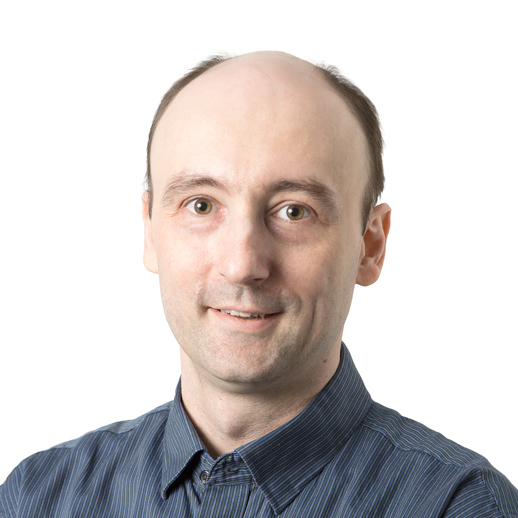
\includegraphics[width = .8in]{figs/figsforpres/stefan.jpg}
    \caption{Stefan Mihalas}
\end{figure}
\begin{itemize}
    \item Julie Harris,Jennifer Whitesell, Karla Hirokawa
    \item You? We are looking for coauthors to review results and suggest improvements.
\end{itemize}

\end{column}
\begin{column}{.33\textwidth}
UW Statistics
\begin{figure}
    \centering
    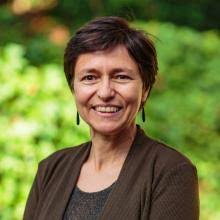
\includegraphics[width = .8in]{figs/figsforpres/meila.jpeg}
    \caption{Marina Meila - Professor of Statistics}
\end{figure}

\begin{figure}
    \centering
    \includegraphics[width = .8in] {figs/figsforpres/koelle_linkedin.png}
    \caption{K - 6th year PhD  (unsupervised learning)}
\end{figure}
\end{column}
\end{columns}
\end{frame}

\begin{frame}{Recent work}
\begin{itemize}
    \item \fullcite{Oh2014-kh}
    \item \fullcite{Harris2016-fn}
    \item \fullcite{Knox2019-ot}
    \item \fullcite{Harris2019-mr}
    \item Paper draft circulated to group (to submit to Network Neuroscience)
\end{itemize}
\end{frame}

\begin{frame}{What remains?}
\begin{itemize}
    \item We would like some more neuroscience context prior to submission
    \item We have anterograde mesoscale connectivity matrices for $117$ cre lines (but not all structures)
    \item Do you have a particular cre-line/source/target of interest? We would like to know!
    \item Previous talk (January) - methodology
    \item This talk - figures from main text of paper and relevant cre/structure info
\end{itemize}
\end{frame}

\begin{frame}{Anterograde tracing experiments}
\begin{columns}
\begin{column}{0.9\textwidth}
\begin{figure}[H]
\subfloat[]{
\label{fig:mouse}
    
\includegraphics[width=0.3\textwidth]{figs/figure1a.png}}
\subfloat[]{
\label{fig:injproj}
    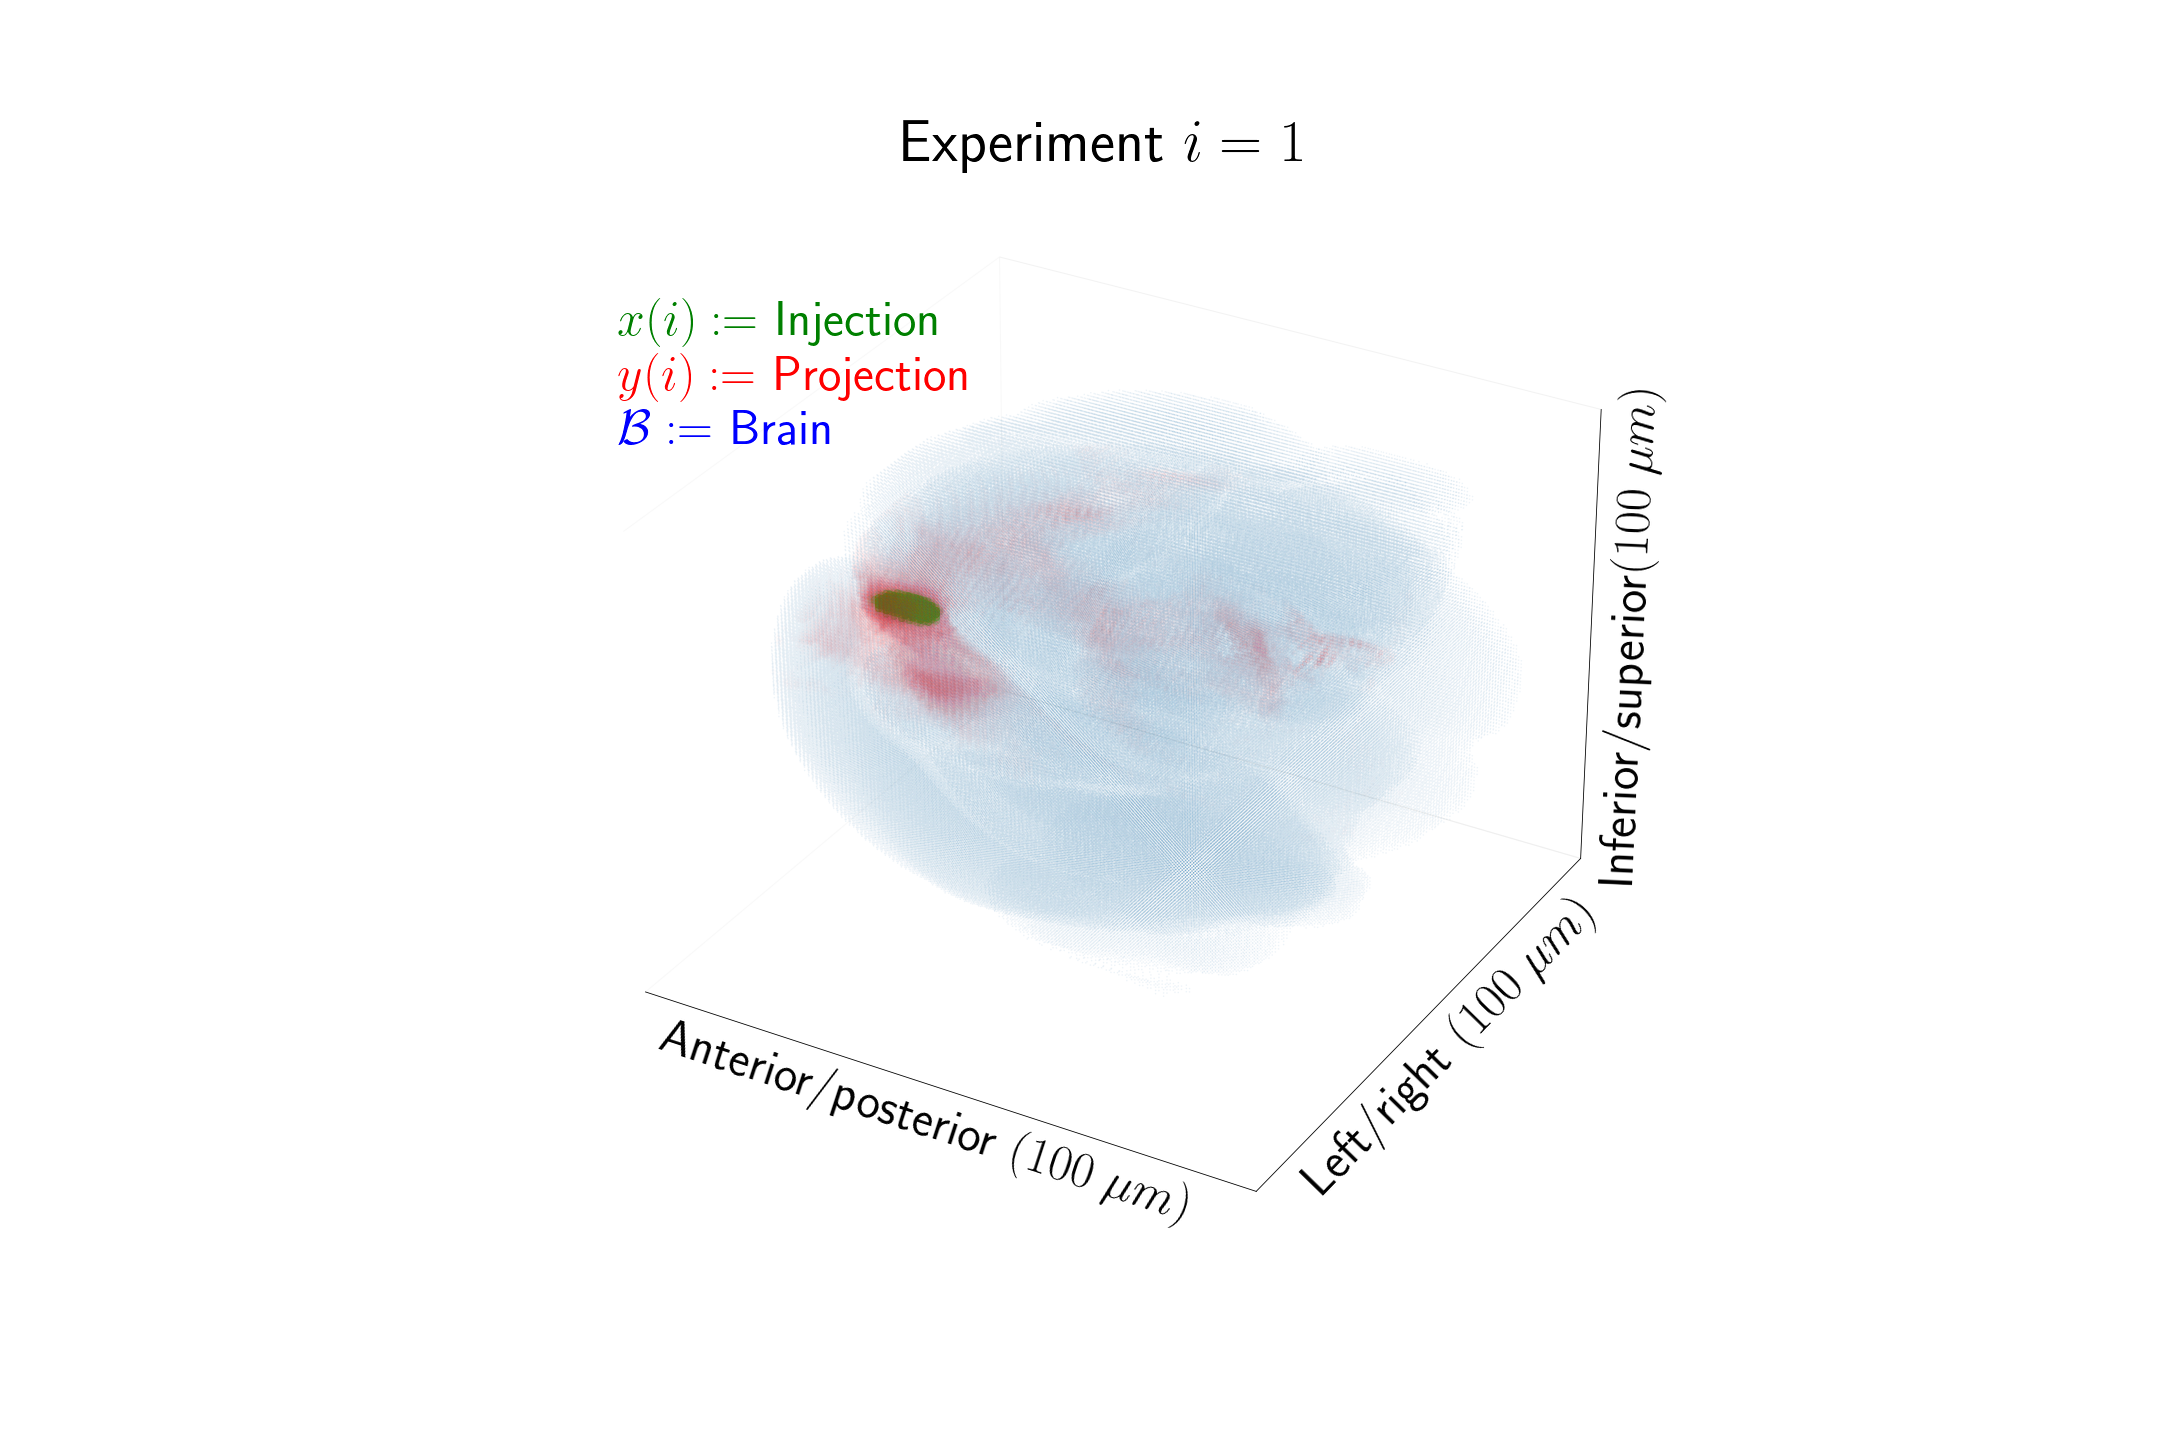
\includegraphics[width=0.4\textwidth]{figs/inj_proj_figure_v2.png}}
\subfloat[]{
\label{fig:segment}
    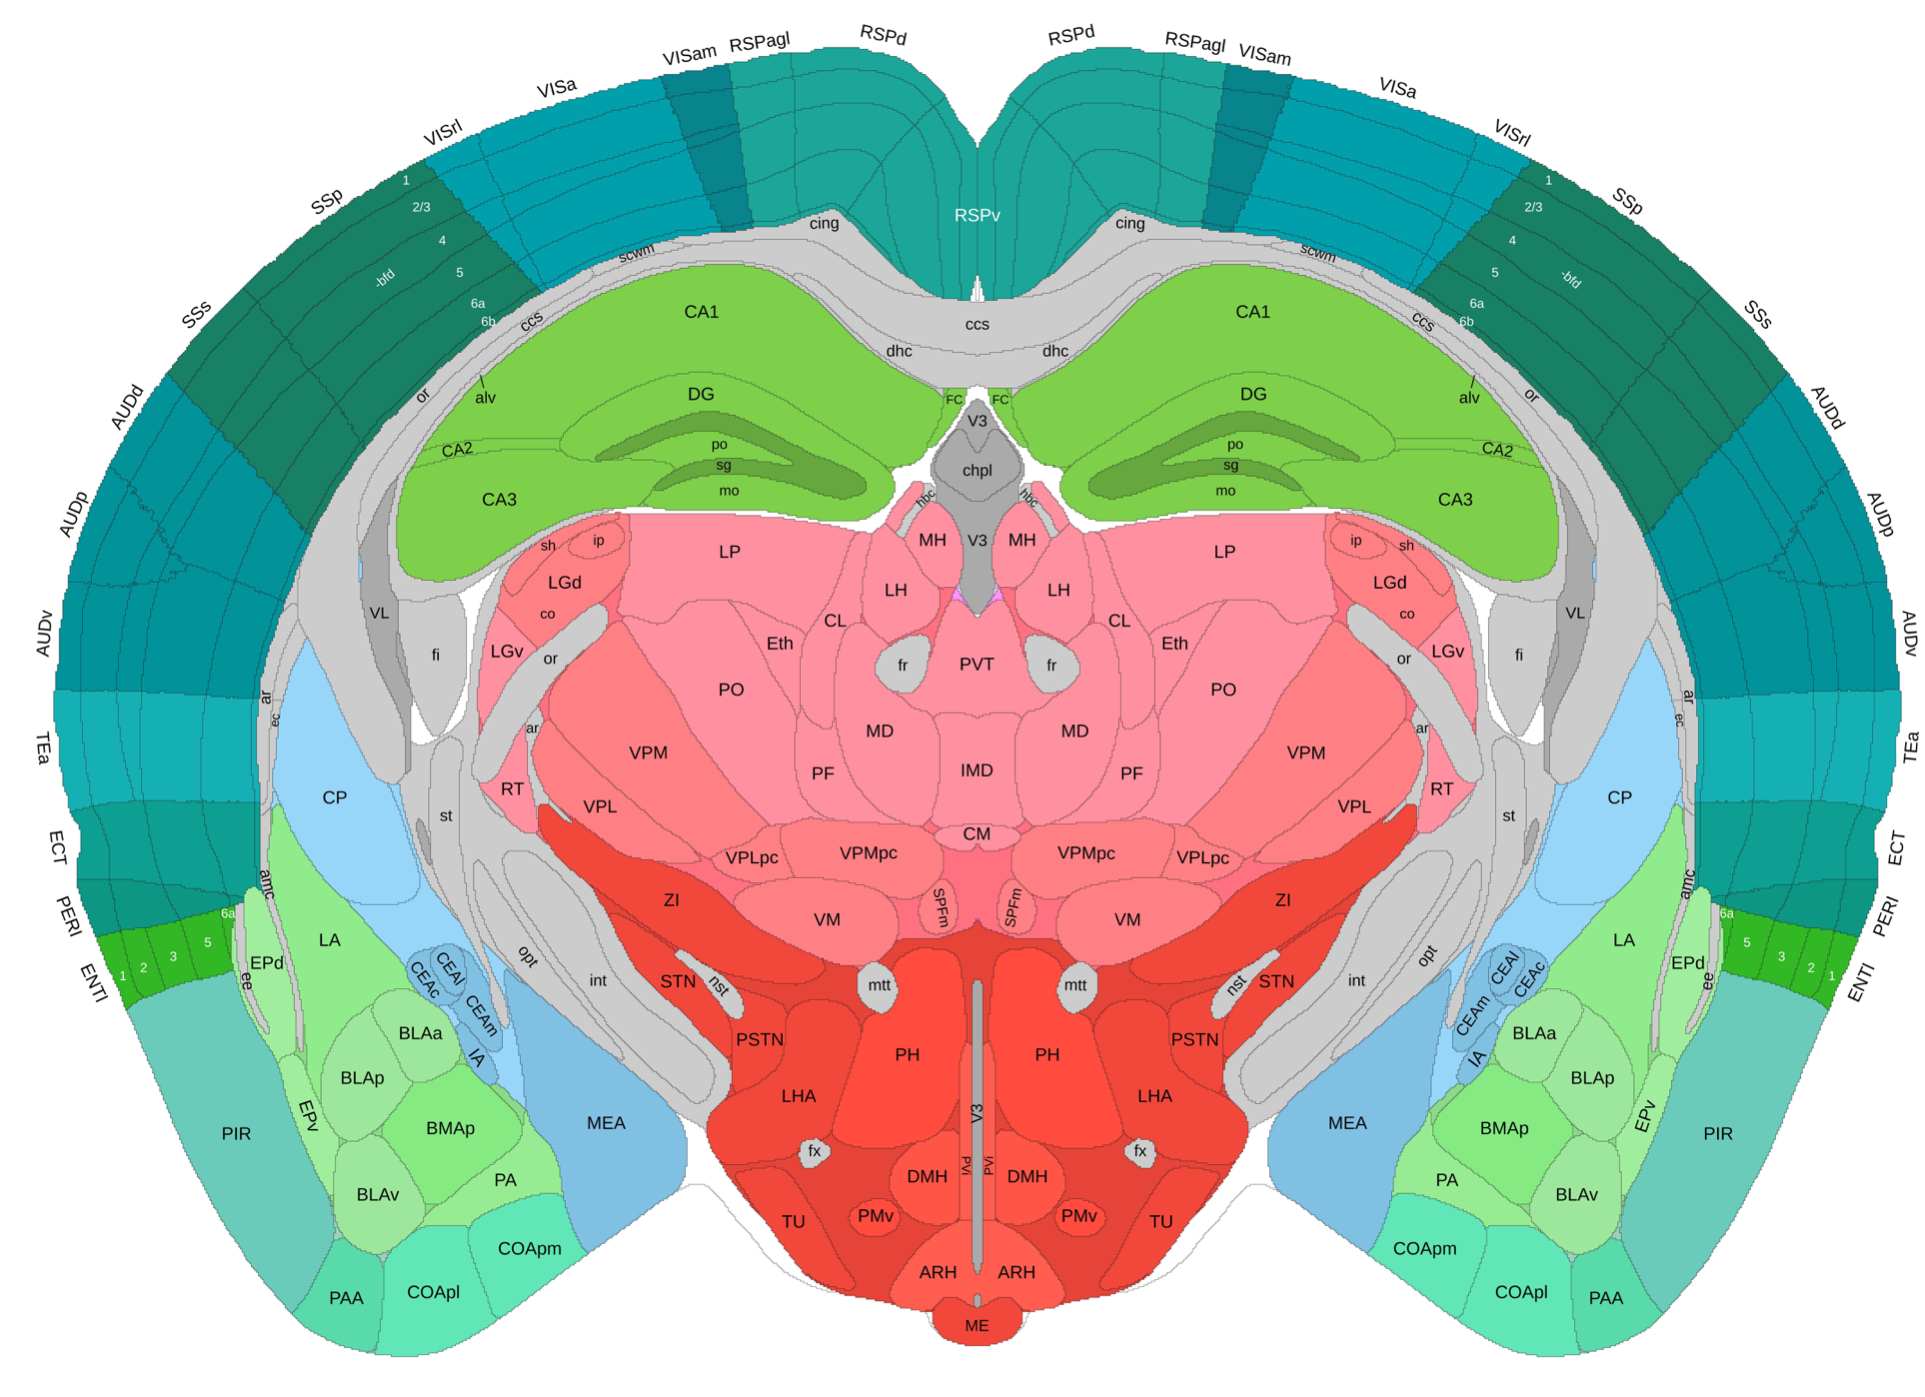
\includegraphics[width=0.3\textwidth]{figs/fig1c.png}}
    \newline
 \subfloat[]{
 \label{fig:ontology}
    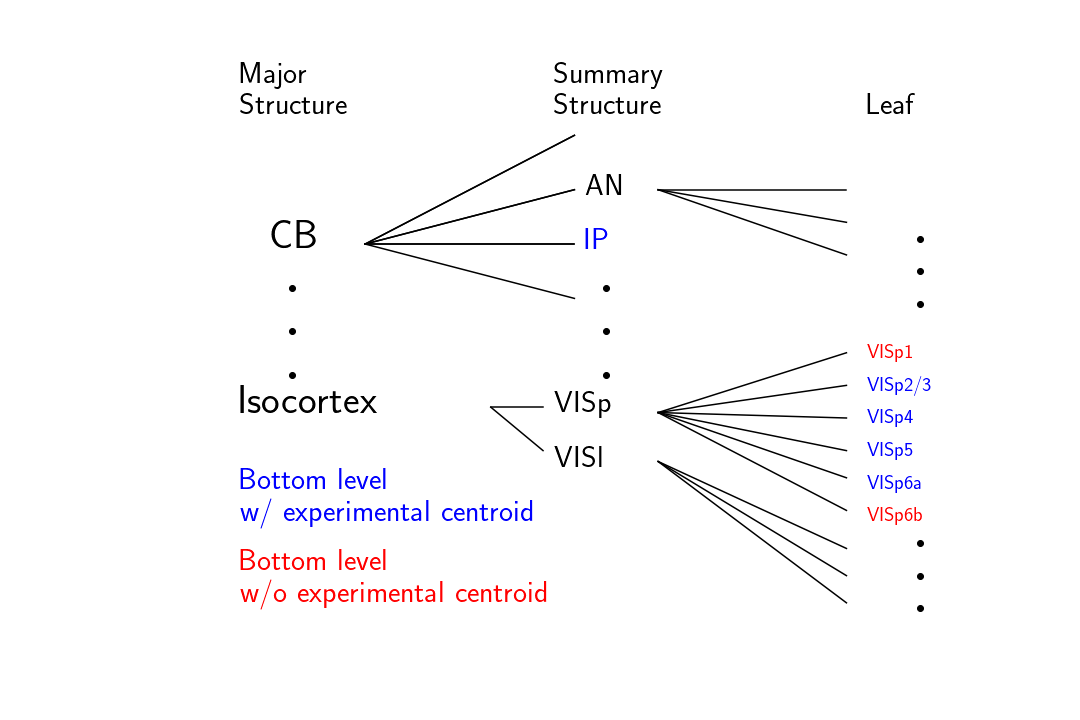
\includegraphics[width=0.35\textwidth]{figs/figsforpres/ontologyfigure.png}}
\subfloat[]{
 \label{fig:top}
    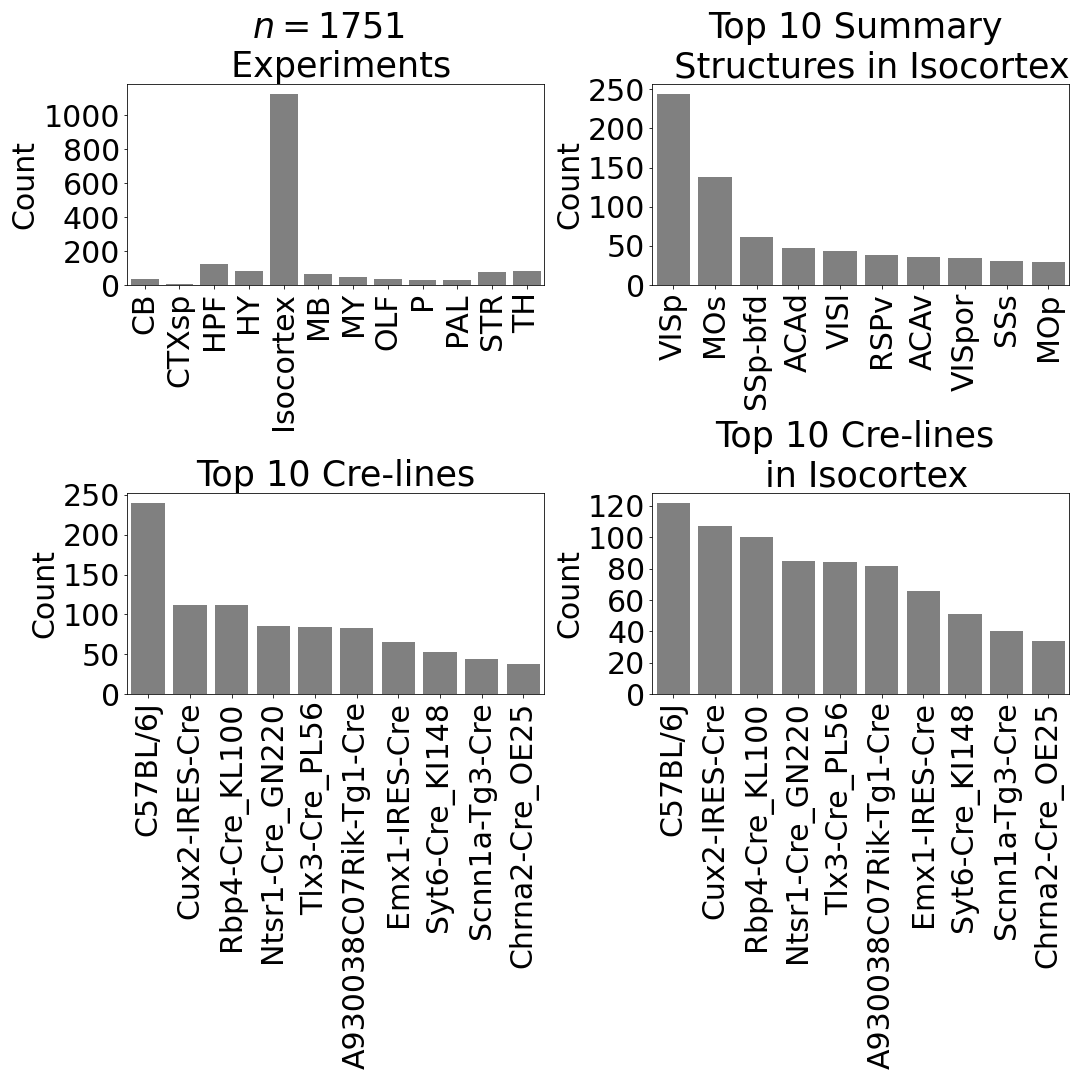
\includegraphics[width=0.35\textwidth]{figs/figsforpres/datasummary.png}}
\subfloat[]{
 \label{fig:combos}
    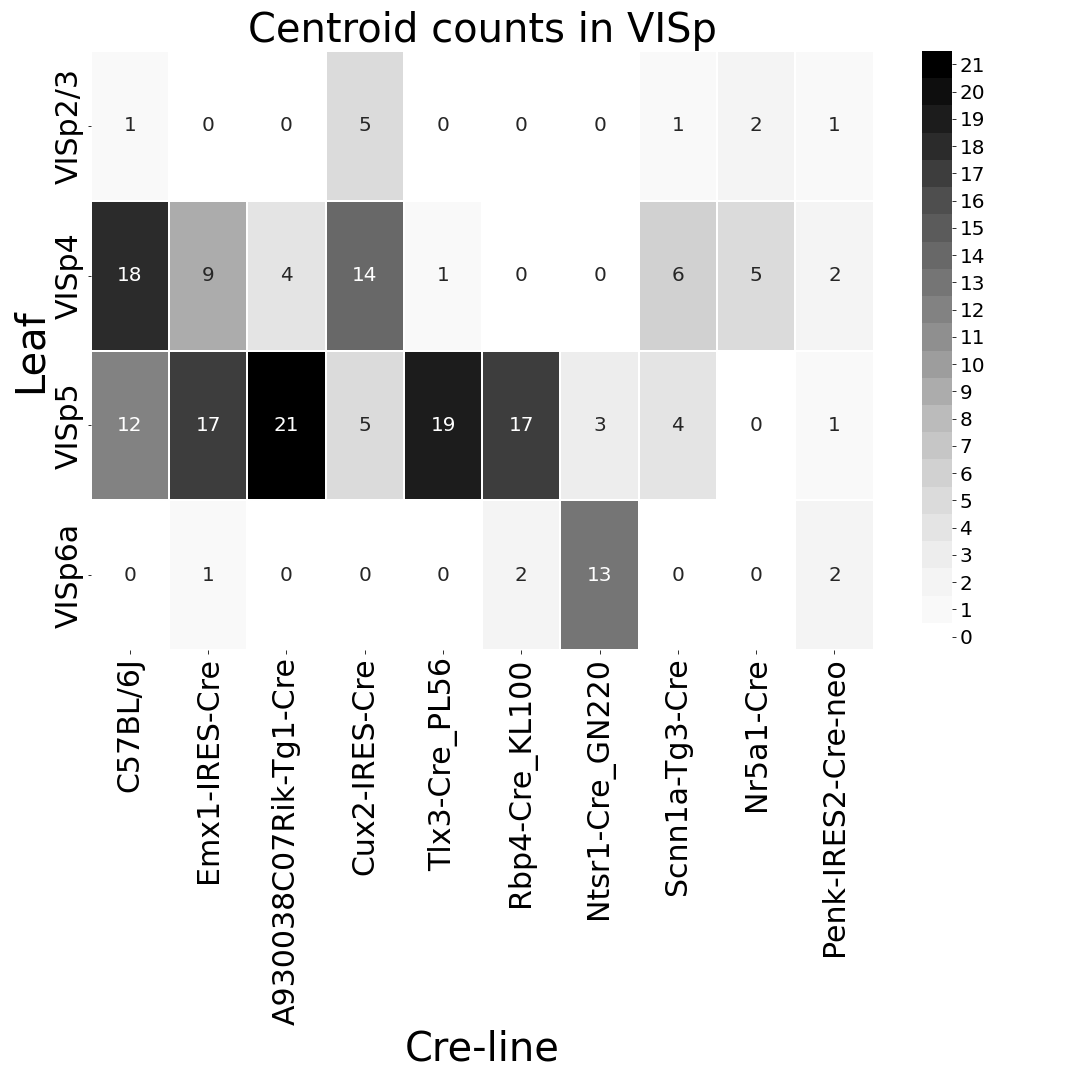
\includegraphics[width=0.35\textwidth]{figs/figsforpres/visp_counts.png}}   
    \label{fig:data}
\end{figure}
\end{column}
\end{columns}
\end{frame}

\begin{frame}{Our goal}
The goal is to use tracing experiments from \citeauthor{Harris2019-mr} to estimate 
\begin{eqnarray*}
\mathcal C: V \times S \times T \to \mathbb R_{\geq 0},
\end{eqnarray*}
the matrix containing connection from \textit{source} $s \in S$ to \textit{target} $t \in T$ observed with virus  $v$.
\end{frame}

\begin{frame}{Connectivities}
\begin{figure}[H]
\centering
    \label{fig:full_wt}
    \includegraphics[width = \textwidth]{analyses/paper/figures/conn_leafs_0617.png}
        \newline
   \end{figure}
\end{frame}

\begin{frame}{Connectivities}
\begin{figure}[H]
\centering
    \label{fig:cortex_wt}
    \includegraphics[width = .5\textwidth]{analyses/paper/figures/conn_sum_cortex_0617.png}
   \end{figure}
\end{frame}


\begin{frame}{Cre-specific targeting}

\begin{figure}[H]
\label{fig:ct_spc}
    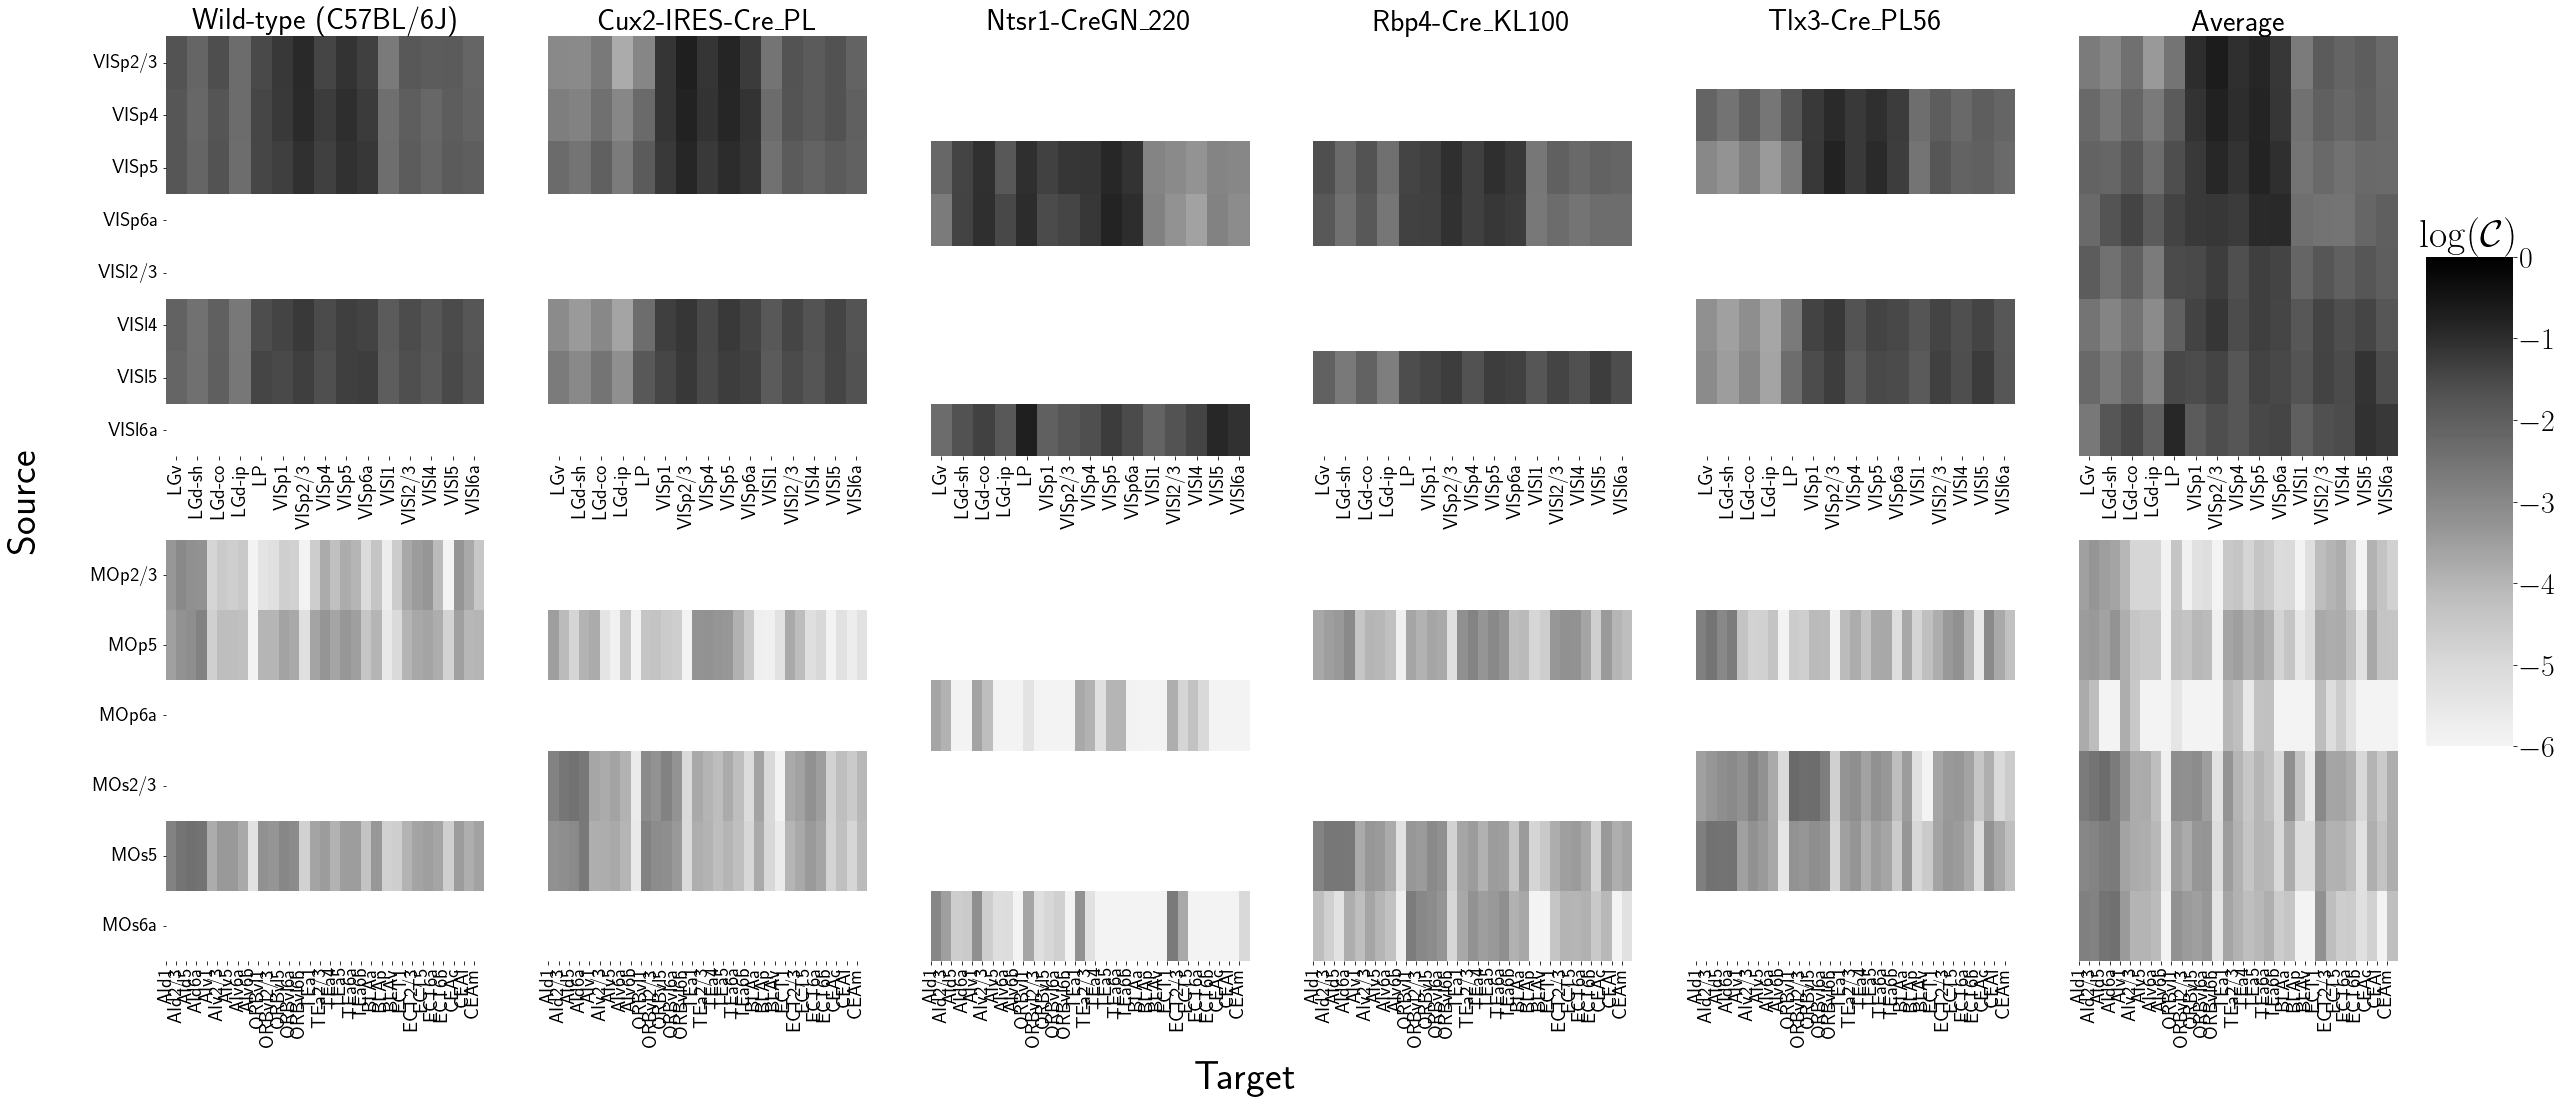
\includegraphics[width=.8\textwidth]{analyses/paper/figures/visp_mo_0615.png} 
\label{fig:data_ct}
\end{figure}
\end{frame}

\begin{frame}{Cre-specific targeting}
\begin{figure}[H]
 \label{fig:ct_clust}
    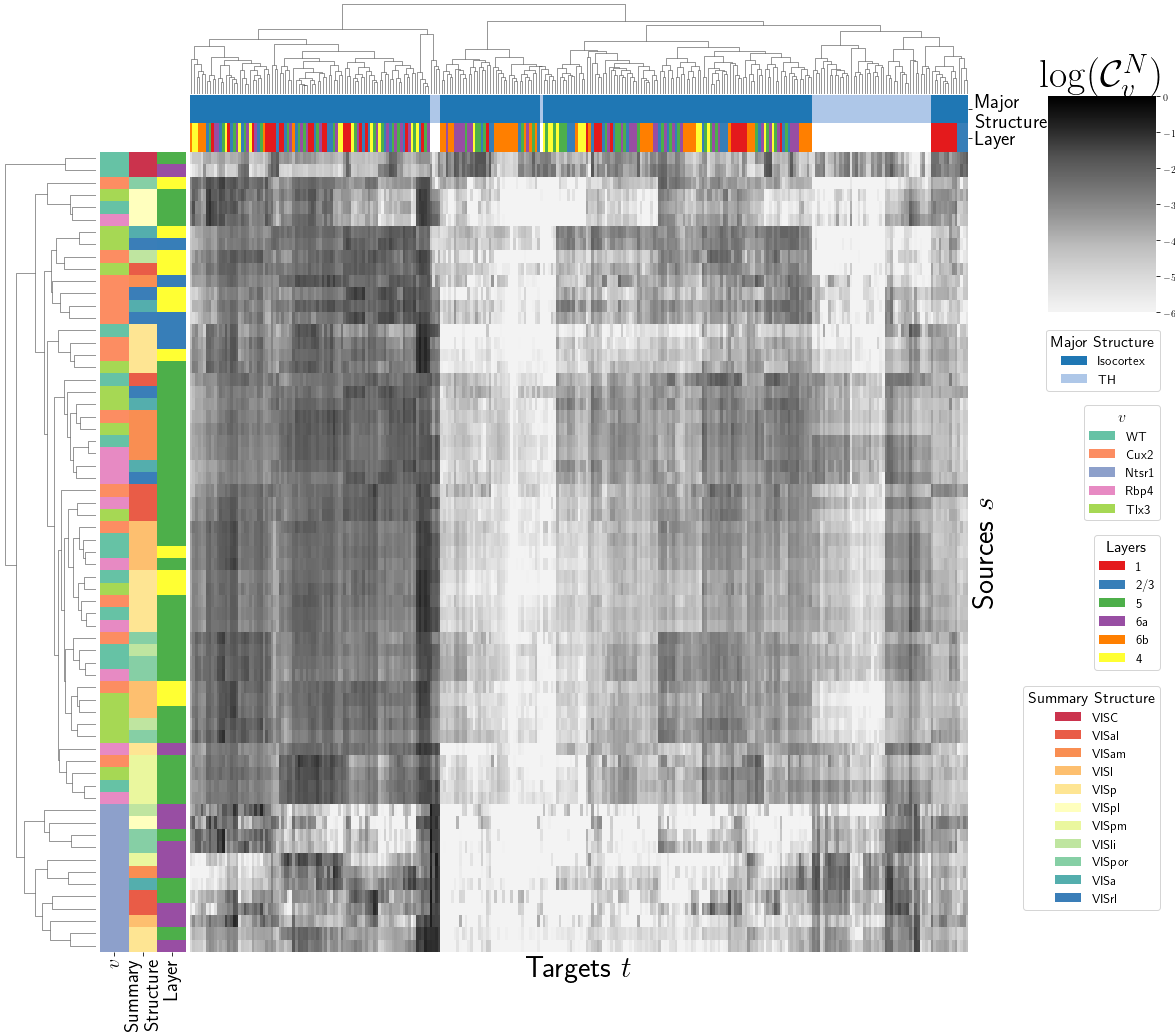
\includegraphics[width=.8\textwidth]{analyses/paper/figures/heirarchical.png}
\label{fig:data_ct}
\end{figure}
\end{frame}

\begin{frame}{Factoring the wild-type connectome}
\begin{eqnarray*}
\mathcal C = WH
\end{eqnarray*}
\begin{figure}[H]
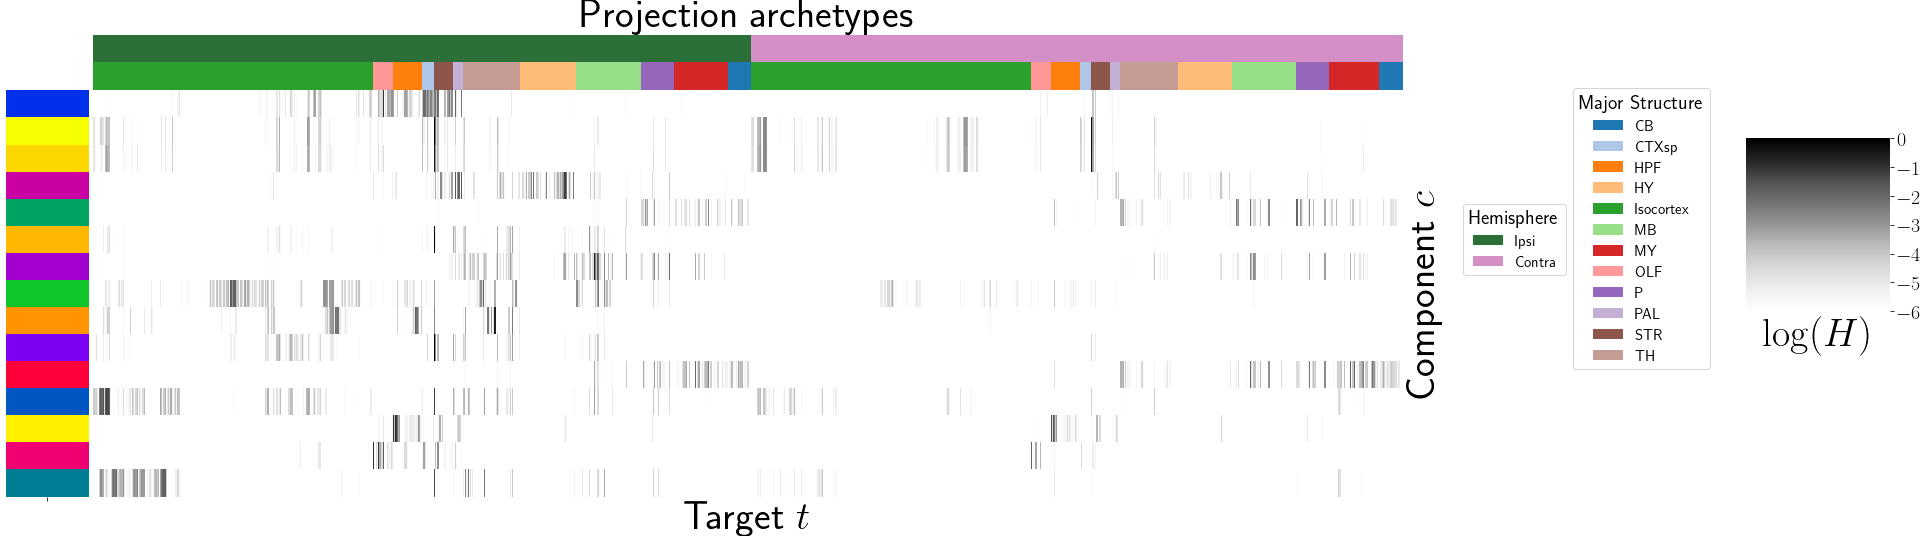
\includegraphics[width =  \textwidth]{paper/figures/H_wt_0617.png}
\label{fig:H}
%\subfloat[]{\includegraphics[width = 1.5in]{figs/figsforpres/test_train.png}} &
\end{figure}
\end{frame}

\begin{frame}{Factoring the wild-type connectome}
\begin{columns}
\begin{column}{.5\textwidth}
\begin{eqnarray*}
\mathcal C = WH
\end{eqnarray*}
\end{column}
\begin{column}{.5\textwidth}
\begin{figure}[H]
\begin{tabular}[t]{c}
\includegraphics[width = .55\textwidth]{paper/figures/W_wt_0617.png}
\label{fig:W}
\end{tabular}
\label{fig:nmf_results}
\end{figure}
\end{column}
\end{columns}
\end{frame}

\begin{frame}{What we need help with}

\begin{itemize}
    \item The statistical methodology and workflow is well-established.
    \item However, the biological inspection of results could use some assistance.
\end{itemize}
\end{frame}


\begin{frame}{Top cre-lines and structures (bold are examined in paper)}
\begin{columns}
\begin{column}{.5\textwidth}
\begin{table}
\small
\begin{tabular}{ll}
Cre-line  & \# experiments   \\
\bm{C57BL/6J }             &  240 \\
\bm{Cux2-IRES-Cre   }      &  112 \\
\bm{Rbp4-Cre\_KL100    }    &  112 \\
\bm{Ntsr1-Cre\_GN220 }      &   86 \\
\bm{Tlx3-Cre\_PL56 }        &   84 \\
A930038C07Rik-Tg1-Cre &   83 \\
Emx1-IRES-Cre         &   66 \\
Syt6-Cre\_KI148        &   53 \\
Scnn1a-Tg3-Cre        &   44 \\
Chrna2-Cre\_OE25       &   38 \\
Efr3a-Cre\_NO108       &   37 \\
Sim1-Cre\_KJ18         &   36 \\
Gpr26-Cre\_KO250       &   25 \\
\end{tabular}
\end{table}
\end{column}
\begin{column}{.5\textwidth}
\begin{table}
\small
\begin{tabular}{ll}
%\toprule
Structure        &   \# experiments   \\
%\midrule
\bm{VISp5}    &  124 \\
\bm{MOs5 }    &  100 \\
\bm{VISp4}    &   75 \\
CP       &   43 \\
ACAd5    &   41 \\
ACAv5    &   33 \\
SSp-bfd5 &   29 \\
\bm{VISp6a}   &   26 \\
AUDp5    &   25 \\
VISpor5  &   24 \\
\bm{MOs2/3}   &   24 \\
VISl5    &   23 \\
RSPv5    &   23 \\
\bm{MOp5 }    &   23 \\
VISam5   &   22 
%\bottomrule
\end{tabular}
\end{table}
\end{column}
\end{columns}
and more... other cre-lines or structures we should look at?
\end{frame}

\begin{frame}{Examine our matrix factorization?}
\begin{itemize}
    \item We are able to learn major structure-specific signals using matrix factorization.
    \item Can we establish a biological correspondence of more subtle signals that we've detected?
\end{itemize}
\end{frame}

\begin{frame}{Thanks!}
\begin{itemize}
\item Questions?
\item Schedule a meeting? (sjkoelle@gmail.com or contact Stefan)
\end{itemize}
\end{frame}


\end{document}
